\documentclass[twocolumn]{article}

\usepackage{listings}
\usepackage{graphicx}

\title{Lab#2\\Computational Physics I - Phys381}
\author{Guilherme Contesini , 10140201 \\ Gerswin Magat , 00325287}

\begin{document}

\maketitle

\newpage

%%%%%%%%%%%%%%%%%%%%%%%%%%%%%%%%%%%%%%%%%%%%%%%%%%%%%%%%%%%%%%%%%%%%%%%%%%%%%%%%%%%%%%%%%%%%%%%%%%%%%%%%%%%%%%%%%%%%%%%%

\section{Fractals}

%%%%%%%%%%%%%%%%%%%%%%%%%%%%%%%%%%%%%%%%%%%%%%%%%%%%%%%%%%%%%%%%%%%%%%%%%%%%%%%%%%%%%%%%%%%%%%%%%%%%%%%%%%%%%%%%%%%%%%%%

\subsection{Question a:}
%%%%%%%%%%%%%%%%%%%%%%%%%%%%%%%%%%%%%%%%%%%%%%%%%%%%%%%%%%%%%%%%%%%%%%%%%%%%%%%%%%%%%%%%%%%%%%%%%%%%%%%%%%%%%%%%%%%%%%%%
\subsubsection{Question a-i:}
A complex number will produce a fractal if, when starting at zero and applying a law(interaction), keeps bounded until the number of interactions break.
The interaction is going to keep bounded if you set a specific value for the complex number. On this interaction law the values for the complex number that keeps the value bounded are $-1<x\leq1$.
\\
\\
Data points obtained from [~\ref{[program-i]}]:\\
\\
\begin{tabular}{|c|c|c|}
\hline
n_c & complex z & $|complex z|^2$\\\hline
1 & ( 0.300, 0.300) & 0.424 \\\hline
2 & ( 0.300, 0.483) & 0.566 \\\hline
3 & ( 0.159, 0.587) & 0.609 \\\hline 
4 & (-2.0E-02, 0.48) & 0.488 \\\hline 
\end{tabular}
%%%%%%%%%%%%%%%%%%%%%%%%%%%%%%%%%%%%%%%%%%%%%%%%%%%%%%%%%%%%%%%%%%%%%%%%%%%%%%%%%%%%%%%%%%%%%%%%%%%%%%%%%%%%%%%%%%%%%%%%
\subsubsection{Question a-ii:}
\\
Data points obtained from [{ ~\ref{[program-ii]} }]:\\
\\
\begin{tabular}{|c|c|c|}
\hline
n_c & complex z & $|complex z|^2$\\\hline
1 & ( 0.500,  1.000) & 1.118 \\\hline  
2 & (-0.250,  2.000) & 2.015 \\\hline  
3 & (-3.437,  0.000) & 3.437 \\\hline 
4 & ( 12.31,  1.000) & 12.35 \\\hline 
5 & ( 151.1,  25.63) & 153.3 \\\hline
\end{tabular}


%%%%%%%%%%%%%%%%%%%%%%%%%%%%%%%%%%%%%%%%%%%%%%%%%%%%%%%%%%%%%%%%%%%%%%%%%%%%%%%%%%%%%%%%%%%%%%%%%%%%%%%%%%%%%%%%%%%%%%%%


%%%%%%%%%%%%%%%%%%%%%%%%%%%%%%%%%%%%%%%%%%%%%%%%%%%%%%%%%%%%%%%%%%%%%%%%%%%%%%%%%%%%%%%%%%%%%%%%%%%%%%%%%%%%%%%%%%%%%%%%

\subsection{Question B:}

Figure obtained through the [{~\ref{main-program}}] and plotted using [~\ref{gnuplot-script}]:\\
\begin{figure}[!h]
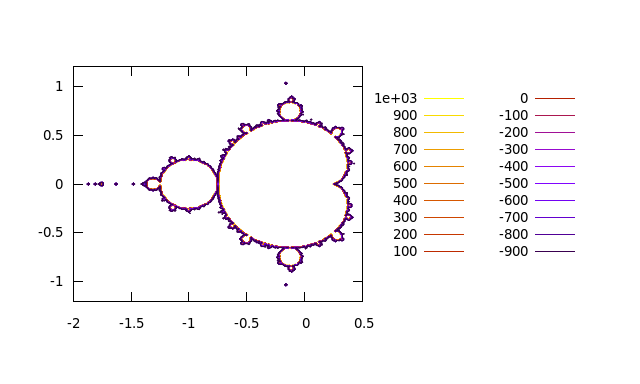
\includegraphics[width=1.1\textwidth]{lab2.png}
\end{figure}

%%%%%%%%%%%%%%%%%%%%%%%%%%%%%%%%%%%%%%%%%%%%%%%%%%%%%%%%%%%%%%%%%%%%%%%%%%%%%%%%%%%%%%%%%%%%%%%%%%%%%%%%%%%%%%%%%%%%%%%%

\newpage

%%%%%%%%%%%%%%%%%%%%%%%%%%%%%%%%%%%%%%%%%%%%%%%%%%%%%%%%%%%%%%%%%%%%%%%%%%%%%%%%%%%%%%%%%%%%%%%%%%%%%%%%%%%%%%%%%%%%%%%%

\subsection{Codes:}

\subsubsection{Question a-i:\\}\label{[program-i]}
\begin{listing}
\begin{indent}
program main\\
  complex :: complex_c , complex_z \\
  integer :: i\\
  complex_z = cmplx(0,0)\\
  complex_c = cmplx(.3,.3)\\
  do i=1,4\\
    complex_z = complex_z * complex_z + complex_c\\
    print*, i ,complex_z , abs(complex_z)\\
  enddo\\
end\\
\\
\end{indent}
\end{listing}

%%%%%%%%%%%%%%%%%%%%%%%%%%%%%%%%%%%%%%%%%%%%%%%%%%%%%%%%%%%%%%%%%%%%%%%%%%%%%%%%%%%%%%%%%%%%%%%%%%%%%%%%%%%%%%%%%%%%%%%%
\noindent\rule{8cm}{0.4pt}
\subsubsection{Question a-ii:\\}\label{[program-ii]}
\begin{listing}
\begin{indent}
program main\\
  complex :: complex_c , complex_z \\
  integer :: i\\
  complex_z = cmplx(0,0)\\
  complex_c = cmplx(.5,1)\\
  do i=0,10\\
    complex_z = complex_z * complex_z + complex_c\\
    print*, i , complex_z , abs(complex_z)\\
  enddo\\
end\\
\end{indent}
\end{listing}

%%%%%%%%%%%%%%%%%%%%%%%%%%%%%%%%%%%%%%%%%%%%%%%%%%%%%%%%%%%%%%%%%%%%%%%%%%%%%%%%%%%%%%%%%%%%%%%%%%%%%%%%%%%%%%%%%%%%%%%%
\noindent\rule{8cm}{0.4pt}
\subsubsection{main-program}\\}\label{main-program}
\begin{listing}
\begin{indent}
program\ main                                   \\             !\ beginning\ of\ the\ code \\
\\
  complex :: complex_c , complex_z               \\          !\ declaration\ of\ complex\ statements\\
  integer :: i , j , k                              \\        !\ declaration\ of\ integer\ statements\\
  real :: x , y                                     \\        !\ declaration\ of\ real\ statements\\
\\
  open(12,file="lab2.dat")                            \\      !\ open\ a\ file\ for\ writing\ the\ data\ points\\
\\
  x=-2.0                                               \\     !\ initial\ value\ for\ x\\
  k=-1000                                               \\    !\ maximum\ value\ for\ iterations\\
  do\ j=-200,200                                         \\    !\ first\ loop\ for\ the\ position\ x\\
    y=-2.0                                              \\    !\ initial\ value\ for\ y\\
    do\ i=-200,200                                        \\   !\ second\ loop\ for\ the\ position\ y\\
      complex_c = cmplx( x , y )                        \\    !\ value\ for\ complex\ C\\
      complex_z = cmplx( .0 , .0 )                     \\     !\ value\ for\ complex\ Z\\
      do\                                               \\     !\ Third\ loop\\
\\
        complex_z = ( complex_z * complex_z ) + complex_c  \\ !\ Equation\ for\ the\ Mandelbrot\\
\\
        if\(abs(complex_z) >= 2.0 )\ then                 \\    !\ first\ condition\ for\ breaking\ the\ loop \\
          exit                                         \\     !\ break\ the\ loop\\
        end\ if                                          \\    !\ end\ of \ the \ condition\\
        if\(k == 1000 )\ then                            \\     !\ second \ condition \ for\\
          exit                                         \\     !\ break \ the \ loop\\
        end\ if                                         \\     !\ end \ of \ the \ condition\\
        k=k+1                                           \\    !\ increments \ for \ the \ number \ of \ iterations\\
      end\ do                                            \\    !\ end \ of \ the \ third \ loop\\
      write(12,*), real(complex_c) , aimag(complex_c) , k \\  !\ writing \ the \ data \ on \ the \ open \ file\\
      k=-1000                                          \\     !\ restatement \ for \ k\\
      y = y + 0.01                                      \\    !\ increments \ for \ position \ y\\
    end\ do                                              \\    !\ end \ of \ the \ second \ loop\\
    x = x + 0.01                                       \\     !\ increments \ for \ position \ x\\
  end\ do                                              \\      !\ end \ of \ the \ first \ loop\\
\\
  close(12)                                      \\           !\ close \ the \ open \ file\\
\\
end\ program\ main                                     \\       !\ end \ of \ the \ program\\
\end{indent}
\end{listing}

%%%%%%%%%%%%%%%%%%%%%%%%%%%%%%%%%%%%%%%%%%%%%%%%%%%%%%%%%%%%%%%%%%%%%%%%%%%%%%%%%%%%%%%%%%%%%%%%%%%%%%%%%%%%%%%%%%%%%%%%
\noindent\rule{8cm}{0.4pt}
\subsubsection{gnuplot-script}\\}\label{gnuplot-script}
\begin{listing}
\begin{indent}
reset\\
set xrange[-2.0:0.5]\\
set yrange[-1.2:1.2]\\
set key outside top right\\
set cntrparam levels auto 25\\
unset ztics\\
set key outside top right\\
unset surface\\
set isosamples 50\\
set view map\\
set palette rgbformulae 33,13,10\\
set contour\\
set ticslevel 0.8\\
set view map
splot 'lab2.dat' u 1:2:3 w lines no title\\
pause -1\\
\\
\end{indent}
\end{listing}
\end{Section}
%%%%%%%%%%%%%%%%%%%%%%%%%%%%%%%%%%%%%%%%%%%%%%%%%%%%%%%%%%%%%%%%%%%%%%%%%%%%%%%%%%%%%%%%%%%%%%%%%%%%%%%%%%%%%%%%%%%%%%%%
\end{document}